\section{Network security protocols}

Communications security must address several critical challenges:
\begin{itemize}
    \item \textit{Trust and integrity}: establishing trust between parties, protecting sensitive data, and ensuring the atomicity of transactions—ensuring each transaction is complete and accurate.
    \item \textit{Protocol limitations}: internet protocols often face issues with authentication and confidentiality.
    \item \textit{Adoption and consistency}: ensuring that security protocols are widely adopted and consistently implemented across different systems and organizations.
\end{itemize}
Two prominent protocols that tackle these challenges are HTTPS (HTTP over SSL/TLS) and SET (Secure Electronic Transaction).
\begin{itemize}
    \item \textit{HTTPS}: Ensures the confidentiality and integrity of communications while allowing for mutual authentication. 
        Despite its strengths, HTTPS does not guarantee how data is used nor does it always enforce strict client authentication in practice.
    \item \textit{SET}: Developed by the VISA and MasterCard consortium, SET focuses on securing transactions rather than just the connections.
        It ensures data usage and transaction security through mechanisms like dual signatures. 
        However, SET struggled with adoption due to scalability issues and the requirement for cardholders to obtain digital certificates. 
        Today, simpler and more scalable methods, such as redirects with tokens to bank websites, are commonly used.
\end{itemize}

\subsection{Transport Layer Security}
TLS, the successor to SSL (Secure Sockets Layer), was developed by the IETF. 
It is designed to ensure:
\begin{itemize}
    \item \textit{Confidentiality and integrity}: protects data during transmission.
    \item \textit{Authentication}: provides server and optional client authentication.
\end{itemize}
TLS uses both symmetric and asymmetric cryptography to balance performance and security. 
The TLS handshake involves the following steps:
\begin{enumerate}
    \item \textit{Client hello}: the client sends a list of supported cipher suites and random data to the server.
    \item \textit{Server hello}: the server responds with the chosen cipher suite, additional random data, and its certificate. 
        The client must verify this certificate.
    \item \textit{Key exchange}: the client sends a pre-master secret encrypted with the server's public key, along with a client certificate if required.
    \item \textit{Secure communication}: an encrypted channel is established for communication.
\end{enumerate}
TLS supports a range of algorithms for key exchange, encryption, digital signatures, and hashing. 
It is designed to be flexible and can adapt to advancements in cryptographic techniques. 
TLS is inherently resistant to MITM attacks, ensuring that only legitimate parties can decrypt and modify data.

TLS offers robust protection for the confidentiality and integrity of transmitted data and authenticates servers and clients.
However, it does not secure data before or after transmission, such as on the server or client side, and it relies on PKI, which can have its own limitations.
The effectiveness of TLS depends on the security and trustworthiness of CAs. 
CAs are responsible for validating domains and organizations and must meet stringent requirements to be included in browser and OS root programs. 
Removing a non-compliant CA can disrupt many websites, making such decisions complex.

\subsection{Secure Electronic Transaction}
SET, a collaborative effort by VISA and MasterCard, was designed to secure transactions by using dual signatures to link order details sent to merchants with payment data sent to payment gateways. 
Despite its innovative approach, SET faced scalability challenges and the complexity of requiring digital certificates for cardholders. 
This hindered its widespread adoption. 
Modern methods, such as token-based redirects to bank websites, have largely replaced SET for secure transactions.
\begin{figure}[H]
    \centering
    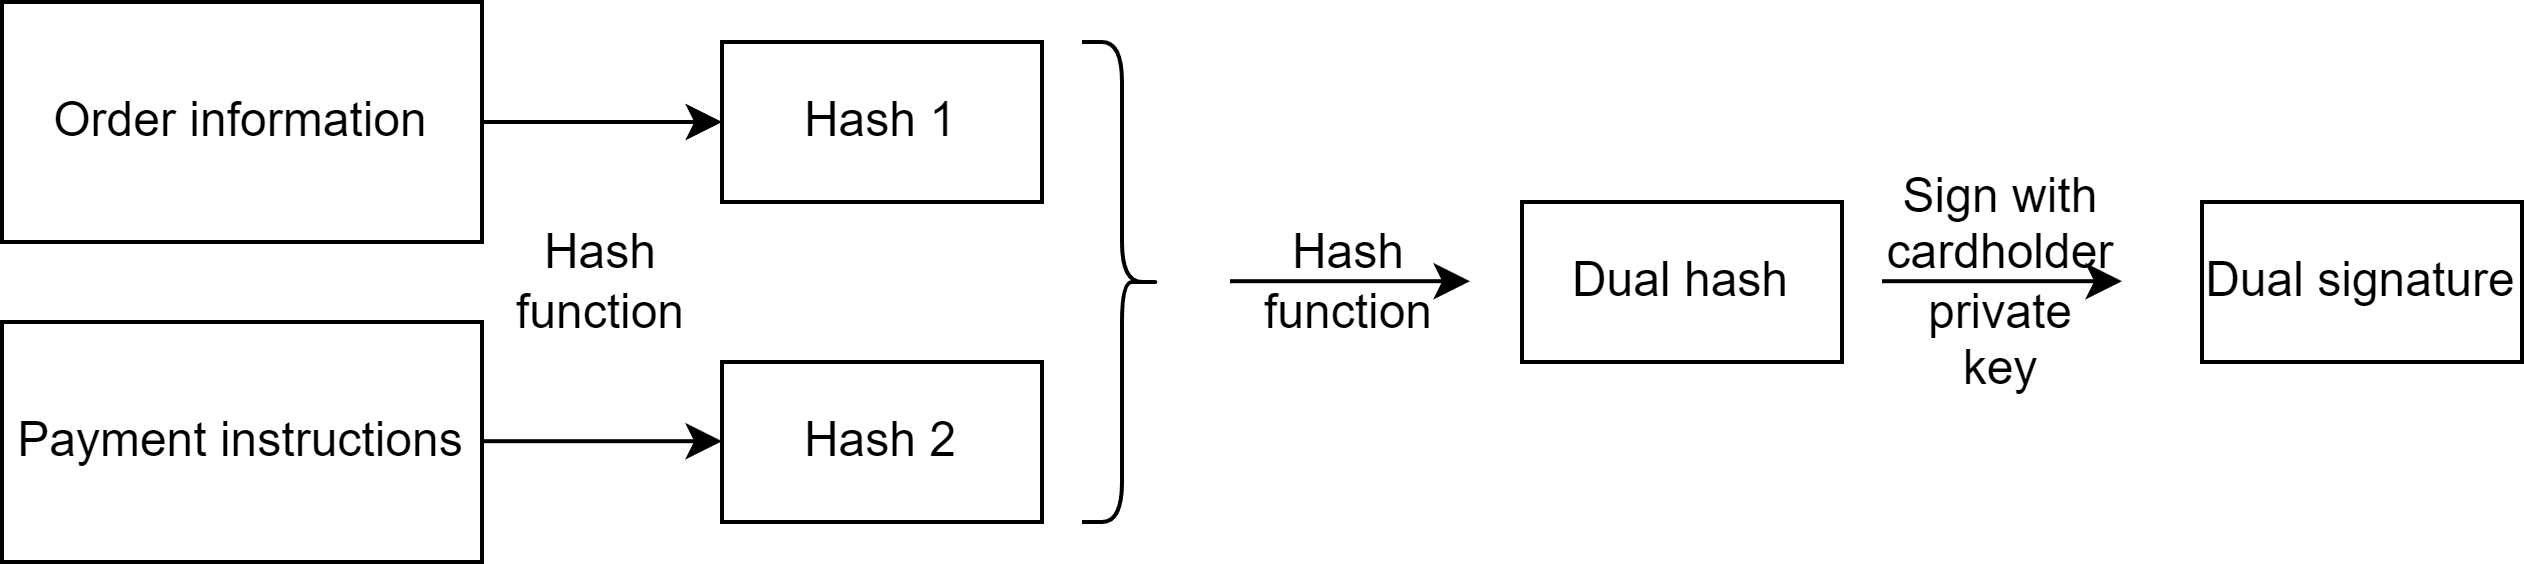
\includegraphics[width=1.0\linewidth]{images/dsg.png}
    \caption{Dual signature generation}
\end{figure}